\section{Diagramme Entité relation}
	\begin{figure}[h!]
       	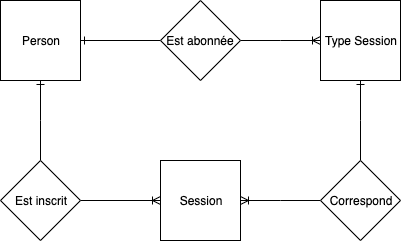
\includegraphics[width=0.8\linewidth, center]{Figures/Entite-relation.png}
       	\caption{Diagramme Relationnel}
	\end{figure}

\newpage
\section{Diagramme Relationnel}
	\begin{figure}[h!]
       	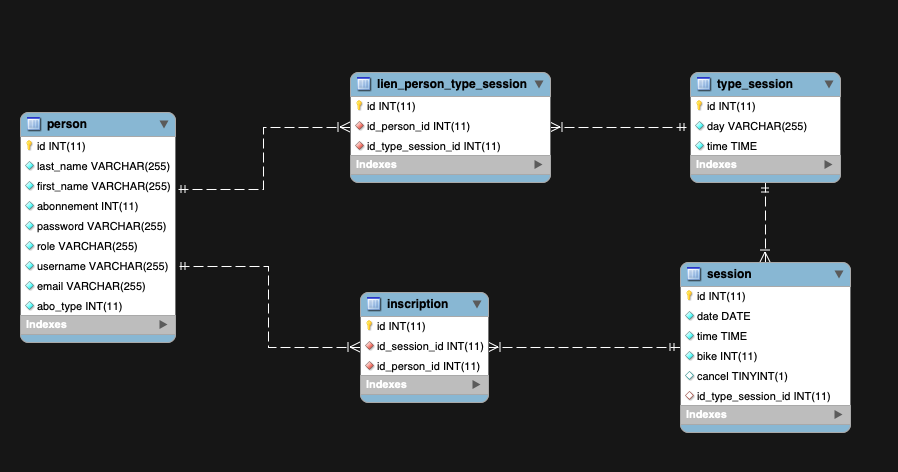
\includegraphics[width=\linewidth, center]{Figures/Diagramme-Relationnel}
       	 \caption{Diagramme Relationnel}
	\end{figure}
	
	
\section{Description des tables et des relations entre tables}
	\paragraph{}
		\begin{tabularx}{\linewidth}{|T{0.15\linewidth}|T{0.15\linewidth}|T{0.15\linewidth}|Y|}
			\hline
			Table & Table & Type & Description\\
			\hline	
			Person & Inscription & 1 à N & Une personne possède plusieurs inscriptions. \\
			\hline
			Session & Inscription & 1 à N & Une session à plusieurs inscriptions. \\
			\hline
			Session & Type Session & N à 1 & Plusieurs sessions corresponde à un type de sessions, un type de session peut correspondre à plusieurs sessions. \\
			\hline
			Person & Lien person type session & 1 à N & Une Personne possède plusieurs liens, plusieurs liens corresponde à une personne. \\
			\hline
			Type Session & Lien person type session & 1 à N & Un type de session possède plusieurs liens, plusieurs liens corresponde à un seul type de session. \\
			\hline
		\end{tabularx}
		
\vspace{\baselineskip}
\section{Description précise des champs}
	\subsection{Table : Person}
		\paragraph{}
			\begin{tabularx}{\linewidth}{|T{0.14\linewidth}|T{0.05\linewidth}|T{0.05\linewidth}|T{0.13\linewidth}|T{0.14\linewidth}|T{0.13\linewidth}|Y|}
				\hline
				Nom & Key & NN & Type & Référence & Intitulé & Commentaire \\
				\hline
				id & PK & O & int & & Identifiant & \\
				\hline
				last\_name & & O & varchar(45) & & Nom & \\
				\hline
				frist\_name & & O & varchar(45) & & Prenom & \\
				\hline
				abonnement & & O & int & & Nombre de session restante & \\
				\hline
				password & & O & varchar(45) & & Mot de passe crypté & \\
				\hline
				role & & O & varchar(45) & & Role sur le site & Default = role\_user \\
				\hline
				username & & O & varchar(45) & & Nom d'utilisateur & Unique \\
				\hline
				email & & O & varchar(45) & & Adresse Email & Unique \\
				\hline
				abo\_type & & O & int & & obonnement origine & \\
				\hline
			\end{tabularx}
	
	
	\subsection{Table : Session}
		\paragraph{}
			\begin{tabularx}{\linewidth}{|T{0.14\linewidth}|T{0.05\linewidth}|T{0.05\linewidth}|T{0.13\linewidth}|T{0.14\linewidth}|T{0.13\linewidth}|Y|}
				\hline
				Nom & Key & NN & Type & Référence & Intitulé & Commentaire \\
				\hline
				id & PK & O & int & & Identifiant & \\
				\hline
				date & & O & DATE & & date & \\
				\hline
				time & & O & Time & & heure & \\
				\hline
				bike & & O & int & & Nombre de vélo restante & \\
				\hline
				cancel & & O & Boolean & & Status de la session & Default = Null\\
				\hline
				id type session & FK & O & int & id / typeSession & Lien avec le type de session & Default = Null\\
				\hline
			\end{tabularx}
			
			
	\vspace{\baselineskip}
	\subsection{Table : Type\_Session}
		\paragraph{}
			\begin{tabularx}{\linewidth}{|T{0.14\linewidth}|T{0.05\linewidth}|T{0.05\linewidth}|T{0.13\linewidth}|T{0.14\linewidth}|T{0.13\linewidth}|Y|}
				\hline
				Nom & Key & NN & Type & Référence & Intitulé & Commentaire \\
				\hline
				id & PK & O & int & & Identifiant & \\
				\hline
				day & & O & varchar(45) & & code du jour & \\
				\hline
				time & & O & Time & & heure & \\
				\hline
			\end{tabularx}
			
			
	\vspace{\baselineskip}
	\subsection{Table : inscription}
		\paragraph{}
			\begin{tabularx}{\linewidth}{|T{0.14\linewidth}|T{0.05\linewidth}|T{0.05\linewidth}|T{0.13\linewidth}|T{0.14\linewidth}|T{0.13\linewidth}|Y|}
				\hline
				Nom & Key & NN & Type & Référence & Intitulé & Commentaire \\
				\hline
				id & PK & O & int & & Identifiant & \\
				\hline
				id\_session & FK & O & int & id / session & lien avec la session & \\
				\hline
				id\_person & FK & O & int & id / person & lien avec la person & \\
				\hline
			\end{tabularx}
			
			
	\vspace{\baselineskip}
	\subsection{Table : lien\_person\_type\_session}
		\paragraph{}
			\begin{tabularx}{\linewidth}{|T{0.2\linewidth}|T{0.05\linewidth}|T{0.05\linewidth}|T{0.06\linewidth}|T{0.15\linewidth}|T{0.13\linewidth}|Y|}
				\hline
				Nom & Key & NN & Type & Référence & Intitulé & Commentaire \\
				\hline
				id & PK & O & int & & Identifiant & \\
				\hline
				id\_type\_session & FK & O & int & id / type\_session & lien avec le type de session & \\
				\hline
				id\_person & FK & O & int & id / person & lien avec la person & \\
				\hline
			\end{tabularx}